
\begin{verbatim}
create table
utente(username varchar(20) primary key, 
nome varchar(20), 
cognome varchar(20), 
indirizzo varchar(50), 
password varchar(20), 
email varchar(20)
); 

\end{verbatim}

\begin{figure}[H]
\centering
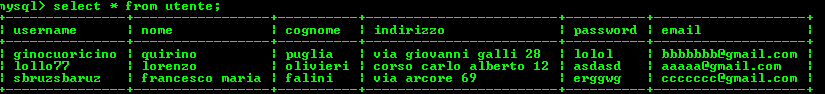
\includegraphics[width=0.7\linewidth]{immagini/1}
\caption{}
\label{fig:1}
\end{figure}

\begin{verbatim}

create table prodotto (codPro int primary key auto_increment, 
descrizione varchar(100), 
prezzo decimal(5,2),
nome varchar(20)
);FOTO2

\end{verbatim}

\begin{figure}[H]
\centering
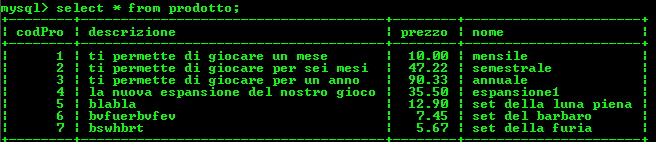
\includegraphics[width=0.7\linewidth]{immagini/2}
\caption{}
\label{fig:1}
\end{figure}

\begin{verbatim}

create table sottoscrizione( 
codSottoscr int primary key auto_increment, 
durata int, 
foreign key (codSottoscr) 
			references prodotto(codPro)
);
\end{verbatim}

\begin{figure}[H]
\centering
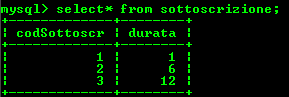
\includegraphics[width=0.7\linewidth]{immagini/3}
\caption{}
\label{fig:1}
\end{figure}

\begin{verbatim}

create table pacchettoOggetti( 
codPacchOgg int primary key auto_increment 
			references prodotto(codPro)
);
\end{verbatim}

\begin{figure}[H]
\centering
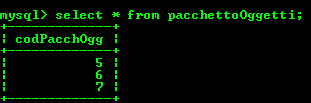
\includegraphics[width=0.7\linewidth]{immagini/4}
\caption{}
\label{fig:1}
\end{figure}

\begin{verbatim}

create table espansione( 
codEsp int primary key auto_increment 
			references prodotto(codPro), 
maxLivello int
);
\end{verbatim}

\begin{figure}[H]
\centering
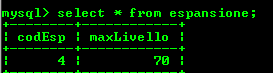
\includegraphics[width=0.7\linewidth]{immagini/5}
\caption{}
\label{fig:1}
\end{figure}

\begin{verbatim}

create table personaggio( 
nome varchar(10) primary key,
razza enum('umano','elfo','nano'), 
classe enum('guerriero','mago','arciere'), 
livello int default 1,
esperienza int default 0,
soldi int default 0, 
capelli enum('capelli1','capelli2','capelli3'), 
colorePelle enum('pelle1','pelle2','pelle3'), 
barba enum('barba1','barba2','barba3'), 
volto enum('volto1','volto2','volto3'), 
puntiVita int, 
puntiMana int, 
attacco int, 
forza int, 
destrezza int, 
intelligenza int, 
xPos int, 
yPos int, 
zPos int
nomeUt varchar(20)
			references utente(username)
);
\end{verbatim}

\begin{figure}[H]
\centering
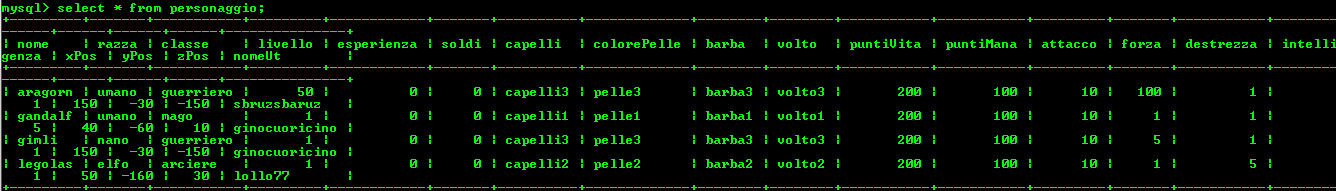
\includegraphics[width=0.7\linewidth]{immagini/6}
\caption{}
\label{fig:1}
\end{figure}

\begin{verbatim}

create table oggetto( 
nome varchar(20) primary key, 
descrizione varchar(50)
);
\end{verbatim}

\begin{figure}[H]
\centering
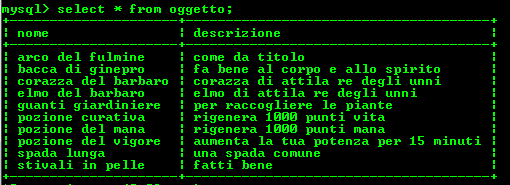
\includegraphics[width=0.7\linewidth]{immagini/7}
\caption{}
\label{fig:1}
\end{figure}

\begin{verbatim}

create table equipaggiamento(
nome varchar(20) primary key 
references oggetto(nome), 
livello int, 
tipo enum(
	'spada', 'ascia', 'mazza',
	'bastone','bacchetta', 'arco', 'balestra','stivale','guanto',
	'corazza','elmo'), 
peso enum('leggera','media','pesante'), 
attacco int, 
difesa int, 
forza int, 
destrezza int, i
ntelligenza int, 
prezzoVendita decimal(5,2), 
prezzoAcquisto decimal(5,2)
);
\end{verbatim}

\begin{figure}[H]
\centering
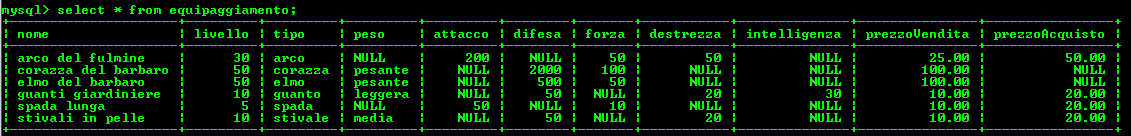
\includegraphics[width=0.7\linewidth]{immagini/8}
\caption{}
\label{fig:1}
\end{figure}

\begin{verbatim}

create table consumabili( 
nome varchar(20) primary key 
			references oggetto(nome), 
livello int, 
puntiVita int, 
puntiMana int, 
attacco int, 
difesa int, 
forza int, 
destrezza int,
intelligenza int, 
prezzoVendita decimal(5,2), 
prezzoacquisto decimal(5,2)
);
\end{verbatim}

\begin{figure}[H]
\centering
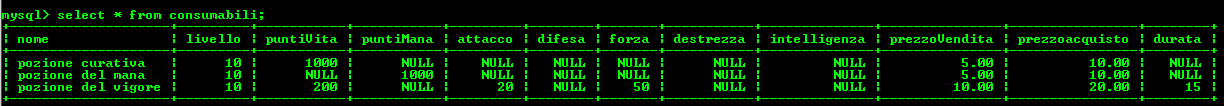
\includegraphics[width=0.7\linewidth]{immagini/9}
\caption{}
\label{fig:1}
\end{figure}

\begin{verbatim}

create table oggettiMissione( 
nome varchar(20) primary key 
			references oggetto(nome)
);
\end{verbatim}

\begin{figure}[H]
\centering
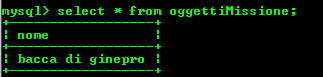
\includegraphics[width=0.7\linewidth]{immagini/10}
\caption{}
\label{fig:1}
\end{figure}

\begin{verbatim}

create table consumo( 
codConsumo int primary key auto_increment, 
dataOra time, 
consumante varchar(20) 
			references personaggio(nome), 
consunto varchar(20) 
			references consumabili(nome)
);
\end{verbatim}

\begin{figure}[H]
\centering
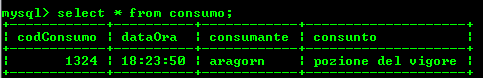
\includegraphics[width=0.7\linewidth]{immagini/11}
\caption{}
\label{fig:1}
\end{figure}

\begin{verbatim}

create table missione( 
codMiss int primary key auto_increment, 
nome varchar(50), descrizione varchar(100), 
livello int, 
completamento bool default FALSE, 
ricompensaOro int, 
ricompensaExp int, 
ricompensaOgg varchar(20) 
			references oggetti(nome), 
xMiss int, 
yMiss int, 
zMiss int
);
\end{verbatim}

\begin{figure}[H]
\centering
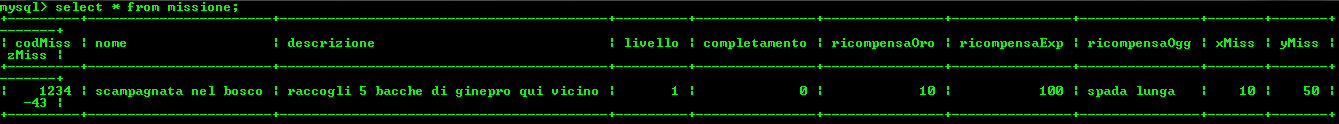
\includegraphics[width=0.7\linewidth]{immagini/12}
\caption{}
\label{fig:1}
\end{figure}

\begin{verbatim}

create table abilità( 
nome varchar(20) primary key, 
descrizione varchar(100),
classe enum('guerriero','mago','arciere'), 
livello int, 
costoMana int, 
attacco int, 
difesa int, 
forza int, 
destrezza int, 
intelligenza int, 
prezzo decimal(5,2)
);
\end{verbatim}

\begin{figure}[H]
\centering
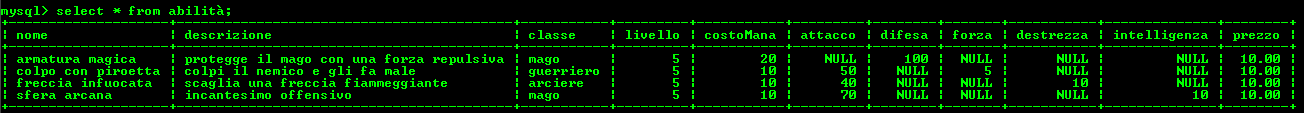
\includegraphics[width=0.7\linewidth]{immagini/13}
\caption{}
\label{fig:1}
\end{figure}

\begin{verbatim}

create table NPCAmichevole( 
nome varchar(20) primary key, 
livello int, 
puntiVita int, 
attacco int, 
difesa int, 
xPos int, 
yPos int, 
zPos int
);
\end{verbatim}

\begin{figure}[H]
\centering
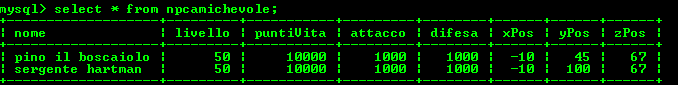
\includegraphics[width=0.7\linewidth]{immagini/14}
\caption{}
\label{fig:1}
\end{figure}

\begin{verbatim}

create table NPCOstile( 
codNPCOST int primary key auto_increment, 
nome varchar(20), 
livello int, 
puntiVita int, 
attacco int, 
difesa int, 
xPos int, 
yPos int, 
zPos int, 
ricompensaOro int, 
ricompensaExp int
);
\end{verbatim}

\begin{figure}[H]
\centering
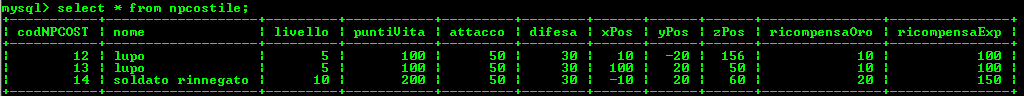
\includegraphics[width=0.7\linewidth]{immagini/15}
\caption{}
\label{fig:1}
\end{figure}

\begin{verbatim}

create table carrello(
nomeUt varchar(50) 
			references utente(username), 
codPro int 
			references prodotto(codPro), 
primary key ( nomeUt, codPro)
);
\end{verbatim}

\begin{figure}[H]
\centering
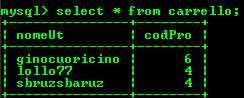
\includegraphics[width=0.7\linewidth]{immagini/16}
\caption{}
\label{fig:1}
\end{figure}

\begin{verbatim}

create table proprietà ( 
nomeUt varchar(50) 
			references utente(username), 
codPro int 
			references prodotto(codPro), 
primary key ( nomeUt, codPro)
);
\end{verbatim}

\begin{figure}[H]
\centering
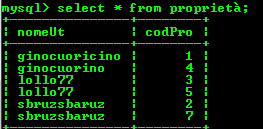
\includegraphics[width=0.7\linewidth]{immagini/17}
\caption{}
\label{fig:1}
\end{figure}

\begin{verbatim}

create table elencazionePacchettoOggetti( 
codPacchOgg int auto_increment 
			references pacchettoOggetti(codPacchOgg), 
oggetto varchar(20)
			references oggetto(nome), 
primary key (codPacchOgg,oggetto)
);
\end{verbatim}

\begin{figure}[H]
\centering
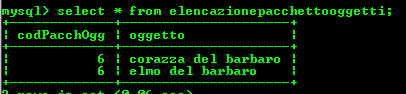
\includegraphics[width=0.7\linewidth]{immagini/18}
\caption{}
\label{fig:1}
\end{figure}

\begin{verbatim}

create table intraprendenza(
personaggio varchar(30) 
			references personaggio(nome), 
missione int  
			references missione(codMiss), 
primary key (personaggio, missione)
);
\end{verbatim}

\begin{figure}[H]
\centering
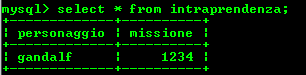
\includegraphics[width=0.7\linewidth]{immagini/19}
\caption{}
\label{fig:1}
\end{figure}

\begin{verbatim}

create table completamento(  
personaggio varchar(30)
			references personaggio(nome), 
missione int  
			references missione(codMiss), 
primary key (personaggio, missione)
);
\end{verbatim}

\begin{figure}[H]
\centering
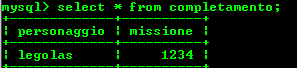
\includegraphics[width=0.7\linewidth]{immagini/20}
\caption{}
\label{fig:1}
\end{figure}

\begin{verbatim}

create table obiettivoAnimato( 
missione int 
			references missione(codMiss), 
nemico int 
			references NPCOstile (codNPCOst), 
primary key (missione,nemico), 
obiettivo int, 
contatore int
);Senza Foto

create table obiettivoInanimato( 
missione int 
			references missione(codMiss), 
oggMiss varchar(20) 
			references oggettiMissione(nome), 
primary key (missione,oggMiss), 
obiettivo int, 
contatore int
);
\end{verbatim}

\begin{figure}[H]
\centering
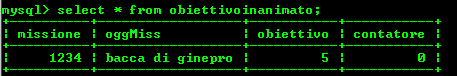
\includegraphics[width=0.7\linewidth]{immagini/21}
\caption{}
\label{fig:1}
\end{figure}

\begin{verbatim}

create table apprendimento(
personaggio varchar(20) 
		references personaggio(nome), 
abilità varchar(20) 
		references abilità(nome), 
primary key(personaggio,abilità)
);

\end{verbatim}

\begin{figure}[H]
\centering
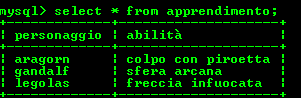
\includegraphics[width=0.7\linewidth]{immagini/22}
\caption{}
\label{fig:1}
\end{figure}

\begin{verbatim}

create table insegnamento(
maestro varchar(20) 
			references NPCAmichevole(nome), 
abilità varchar(20) 
			references abilità(nome), 
primary key(maestro,abilità)
);
\end{verbatim}

\begin{figure}[H]
\centering
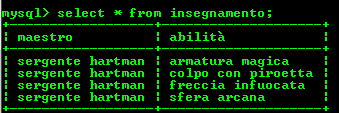
\includegraphics[width=0.7\linewidth]{immagini/23}
\caption{}
\label{fig:1}
\end{figure}

\begin{verbatim}

create table proprietàNPCAmichevole( 
venditore varchar(20) 
			references NPCAmichevole (nome), 
oggetto varchar(20) 
			references oggetto(nome), 
primary key (venditore,oggetto)
);
\end{verbatim}

\begin{figure}[H]
\centering
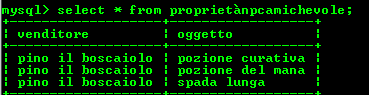
\includegraphics[width=0.7\linewidth]{immagini/24}
\caption{}
\label{fig:1}
\end{figure}

\begin{verbatim}

create table proprietàNPCOstile( 
nemico int 
			references NPCOstile (codNPCOst), 
oggetto varchar(20) 
			references oggetto(nome), 
primary key (nemico,oggetto)
);
\end{verbatim}

\begin{figure}[H]
\centering
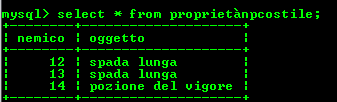
\includegraphics[width=0.7\linewidth]{immagini/25}
\caption{}
\label{fig:1}
\end{figure}

\begin{verbatim}

create table stock( 
personaggio varchar(20) 
			references personaggio(nome), 
oggetto varchar(20)
			references oggetto(nome),
primary key (personaggio,oggetto)
);
\end{verbatim}

\begin{figure}[H]
\centering
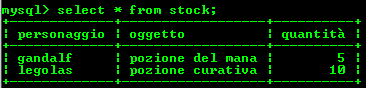
\includegraphics[width=0.7\linewidth]{immagini/26}
\caption{}
\label{fig:1}
\end{figure}

\begin{verbatim}

create table indossamento( 
personaggio varchar(20) 
			references personaggio(nome), 
oggEquip varchar(20) 
			references equipaggiamento(nome),
primary key (personaggio,oggEquip)
);FOTO29
\end{verbatim}

\begin{figure}[H]
\centering
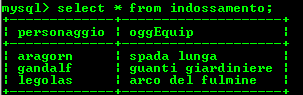
\includegraphics[width=0.7\linewidth]{immagini/27}
\caption{}
\label{fig:1}
\end{figure}

\begin{verbatim}

create table transazione(
codTrans int auto_increment primary key,
dataOra time, 
importo decimal(5,2), 
compratoreReale varchar(20) 
			references personaggio(nome), 

venditoreReale varchar(20) 
			references personaggio(nome), 
compratorePC varchar(20) 
			references NPCAmichevole(nome), 
venditorePC varchar(20) 
			references NPCAmichevole(nome)
);

\end{verbatim}

\begin{figure}[H]
\centering
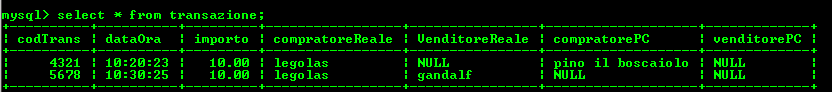
\includegraphics[width=0.7\linewidth]{immagini/28}
\caption{}
\label{fig:1}
\end{figure}

\begin{verbatim}
create table ElencazioneTransazione( 
transazione int 
			references transazione(codTrans), 
oggetto varchar(20)
			references oggetto(nome), 
primary key(transazione,oggetto)
);
\end{verbatim}

\begin{figure}[H]
\centering
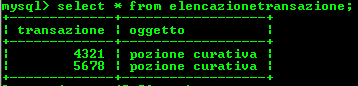
\includegraphics[width=0.7\linewidth]{immagini/29}
\caption{}
\label{fig:1}
\end{figure}

\begin{verbatim}

create table cartaCredito( 
numero int primary key, 
cvv int, 
scadenza date, 
nomeUt varchar(20) 
		references utente(username)
);
\end{verbatim}

\begin{figure}[H]
\centering
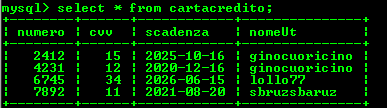
\includegraphics[width=0.7\linewidth]{immagini/30}
\caption{}
\label{fig:1}
\end{figure}

\begin{verbatim}

\end{verbatim}
